\begin{figure}[!htbp]
    \center{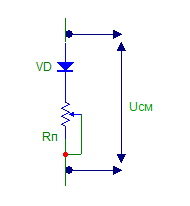
\includegraphics[width=0.4\linewidth]{picture_thermo_1}}
    \caption{Схема цепи термостабилизации на диоде}
    \label{figure:p2_2}
  \end{figure}


На рисунке \ref{figure:p2_1} цепь термостабилизации обозначена как Rt . В данном усилителе будем использовать схему термостабилизации на диоде  (рисунок \ref{figure:p2_2}).
Диоды при этом обязательно должен иметь надежный тепловой контакт с радиатором, на котором установлены выходные транзисторы, иначе термостабилизации  попросту  не  будет.
Данная схема обеспечивает достаточную  температурную стабильность в диапазоне температур $0\ldots +40~^0C$. \par